% !TeX root = ../main.tex
\chapter[Large-Scale Validation of GPU Memory Consistency and Security]{Large-Scale Validation of GPU Memory Consistency and Security}
\label{chap:gpuharbor}

\epigraph{\textit{"It never gets easier, you just go faster."}}{--- Greg Lemond}

\section{Personal Context}

\section{Introduction}

This chapter presents a large-scale study of GPU MCS testing, which tests $10\times$ more devices than previous studies. The techniques that enable this study also are applied in two other ways: (1)~a deep investigation of the MCS implemented by NVIDIA's A100, H100, and GH200 GPUs (\mysec\ref{sec:gpuharbor-nvidia-mcs}), and (2)~an investigation into how observations of weak behaviors can be used to create a low-bandwidth GPU side-channel, which also provided the foundation for the creation of a more sophisticated side-channel across NVIDIA MIG instances on an A100 GPU (\mysec\ref{sec:gpuharbor-sidechannel}).

\paragraph{GPUHarbor.} \myfiglong\ref{tab:gpuharbor-gpu-overview} summarizes the large-scale study, including the number of GPUs tested (\totalDevices), broken down by two frameworks (WebGPU and Vulkan) and seven vendors (Intel, Apple, NVIDIA, AMD, Arm, Qualcomm, and Imagination). This scale is empowered by \gpuharbor, a new cross-platform GPU MCS testing tool suite.  \gpuharbor includes two front-ends, a browser web app (using WebGPU) and an Android app (using Vulkan). The web app was advertised on campus forums and social media to obtain a significant number of WebGPU results. Fewer Vulkan devices are tested as the Android app was not published on the Google Play Store.

As does the work in the previous chapter, \gpuharbor uses litmus tests to evaluate MCS behaviors. Existing GPU MCS testing tools execute litmus tests many times in succession to check conformance and characterize devices~\cite{gpu-exposing, gpu-concurrency, gpu-foundations}. However, these prior approaches have several shortcomings: (1)~they are implemented in vendor-specific languages, e.g., CUDA; (2)~they require  expert users to build, configure, and execute tests on each device, e.g., as is the case for OpenCL; or (3)~litmus tests were embedded in vendor-specific stress testing environments and thus, would not execute efficiently on other devices. This cumbersome litmus testing workflow made it infeasible to perform a large-scale study.  In contrast, \gpuharbor defines litmus tests using a neutral configuration (written in JSON), which it compiles to a portable shading language (WGSL~\cite{webgpu-sl} or SPIR-V~\cite{spir-v}). The resulting litmus testing application then tunes the testing stress automatically. The net result is a fully automated and easy-to-use tool for GPU MCS testing at large. \mytablong\ref{tab:gpuharbor-gpu-overview} shows how many weak memory litmus test iterations were run and how many weak behaviors were observed in the study.

The data set supports the following two investigations: (1)~an examination of MCS conformance test results that finds two new bugs in mobile device GPUs from Arm and NVIDIA, and (2)~a characterization of weak memory behavior profiles, e.g., the rates at which allowed weak behaviors occur and their sensitivity to system stress. Additionally, several analyses are performed on the weak memory profiles. First, per-vendor average profiles are compared; for example, AMD shows an average percentage of 1.5\% weak behaviors, while Intel shows only .06\%. Different GPUs are then clustered, revealing that, surprisingly, cross-vendor devices often have similar profiles, while devices from the \textit{same} vendor sometimes have vastly different profiles. Finally, the wide range of observed profiles is discussed in terms of its impact on testing strategies and the implementation of synchronization algorithms.

\subsection{Contributions}

In summary, the contributions of this chapter are:
\begin{enumerate}
    \item \textbf{Tooling}: \gpuharbor, a new cross-platform GPU MCS testing tool with accessible web and Android interfaces (\mysec\ref{sec:gpuharbor-sys-overview}).

    \item \textbf{GPU MCS Weak Behavior Characterization}: A large GPU weak memory characterization and conformance testing study, collecting data from \totalDevices GPUs (\mysec\ref{sec:gpuharbor-wb-char}).

    \item \textbf{Conformance Testing and Analysis}:
        \begin{enumerate}
            \item The discovery of two unreported bugs in Arm and NVIDIA devices (\mysec\ref{sec:gpuharbor-vulkan-bugs}).
            \item An analysis of statistical similarities across GPUs and a description of the impact on testing strategies and device fingerprinting (\mysec\ref{sec:gpuharbor-webgpu-sim}).
            \item A discussion on how weak behavior profiles impact the development and testing of synchronization algorithms on GPUs (\mysec\ref{sec:gpuharbor-vulkan-locks}).
        \end{enumerate}
    \item \textbf{Lessons Learned: } A set of lessons learned while designing and running this study, providing a guide to other researchers seeking to implement similar large experimental explorations (\mysec\ref{sec:gpuharbor-lessons-learned}).

    %\item \textbf{Pedagogical Impacts}: We show how our tool, \gpuharbor, can be used as a pedagogical tool for teaching students parallel GPU programming, <TYLER WRITE SOME MORE HERE>.
\end{enumerate}

%All of the data we collected as part of the large-scale study, and the tools used to do so, are available as part of our artifact~\cite{gpuharbor-artifact}. In addition, \gpuharbor's web interface is hosted by UC Santa Cruz and can be found at \url{https://gpuharbor.ucsc.edu/webgpu-mem-testing/}.

\newcommand{\exchangelock}{
    \begin{tabular}{l l}
    \multicolumn{2}{c}{Initialize: \texttt{x = 0;}} \\
    \midrule
    \underline{thread 0} & \underline{thread 1} \\
        \texttt{...critical section} & \\
        \texttt{fence(release);} & \texttt{while(EXCHG(x, 1) == 1);} \\
        \texttt{S(x, 0);} & \texttt{fence(acquire);} \\
        & \texttt{...critical section} \\
        \midrule
    \end{tabular} \hspace{1cm}
}

\begin{table}
\centering
\footnotesize
\caption{The GPU vendors and devices included in the study. Overall, almost 400 billion iterations of weak memory tests were run on \totalDevices devices, of which \uniqueDevices were confirmed to be unique models. Over 35 million weak behaviors were observed, with the rates per device and vendor characterized in \mysec\ref{sec:gpuharbor-wb-char}.}
\scalebox{.97}{\begin{tabular}{ l l r r r}
 \toprule
 \textbf{Framework} & \textbf{Vendor} & \textbf{Devices (Unique)} & \textbf{Tests} & \textbf{Weak Behaviors} \\
 \midrule
 \multirow{4}{*}{WebGPU} & Intel & 26 (17) & 105.3b & 0.2m \\
& Apple & 26 (6) & 104.4b & 9.7m \\
& NVIDIA & 31 (18) & 125.3b & 10.8m \\
& AMD & 15 (9) & 60.4b & 14.7m \\
 \midrule
\multirow{4}{*}{Vulkan} & Arm & 2 (2) & 51.6m & 18.2k\\
                 & Qualcomm & 4 (4) & 17.6m & 27.2k\\
                 & Imagination & 1 (1) & 6.1m & 0\\
                 & NVIDIA & 1 (1) & 49.6m & 454\\
\midrule
 & & \textbf{Total: \totalDevices (\uniqueDevices)} & \textbf{395.5b} & \textbf{35.4m} \\
\bottomrule
\end{tabular}}
\label{tab:gpuharbor-gpu-overview}
\end{table}

\newcommand{\mplitmustest}{
    \begin{tabular}{l l}
    \multicolumn{2}{c}{Initialize: \texttt{x = 0; y = 0;}} \\
    \midrule
    \underline{thread 0} & \underline{thread 1} \\
        \circledBlack{\vphantom{A}a}\hspace{.1cm} \texttt{S(x, 1);} &  \circledWhite{\vphantom{A}c}\hspace{.1cm} \texttt{r0 = L(y);}  \\
        \circledBlack{\vphantom{A}b}\hspace{.1cm} \texttt{S(y, 1);} &
        \circledWhite{\vphantom{A}d}\hspace{.1cm} \texttt{r1 = L(x);}  \\
        \midrule
        \multicolumn{2}{c}{Weak Behavior: \texttt{r0 == 1 \&\& r1 == 0}}
    \end{tabular} \hspace{.2cm}
}

\newcommand{\mpcolitmustest}{
    \begin{tabular}{l l}
    \multicolumn{2}{c}{Initialize: \texttt{x = 0;}} \\
    \midrule
    \underline{thread 0} & \underline{thread 1} \\
        \circledBlack{\vphantom{A}a}\hspace{.1cm} \texttt{S(x, 1);} &  \circledWhite{\vphantom{A}c}\hspace{.1cm} \texttt{r0 = L(x);}  \\
        \circledBlack{\vphantom{A}b}\hspace{.1cm} \texttt{S(x, 2);} &
        \circledWhite{\vphantom{A}d}\hspace{.1cm} \texttt{r1 = L(x);}  \\
        \midrule
        \multicolumn{2}{c}{Weak Behavior: \texttt{r0 > r1}}

    \end{tabular}
}

\begin{figure}
\footnotesize
\captionsetup[subfigure]{width=.49\columnwidth}
\subfloat[MP Litmus Test]{\mplitmustest \label{fig:gpuharbor-mp-litmustest}}
\subfloat[MP-CO Litmus Test]{\mpcolitmustest \label{fig:gpuharbor-mp-co-litmustest}} \\
\caption{The weak behavior in the MP litmus test is allowed by many relaxed MCSs. On the other hand, the weak behavior in the closely-related MP-CO litmus test violates coherency and is disallowed by every known major MCS. Prior work~\cite{mc-mutants} has shown that tuning system stress for the allowed MP test can be used to design effective tests for finding bugs related to the MP-CO test.}
%One of our contributions is to scale the approach of previous work~\cite{mc-mutants}, collecting data on the rate of MP weak behaviors and using the results to find violations of MP-CO on GPUs from two vendors.}
\label{fig:gpuharbor-intro-examples}
\end{figure}

\begin{figure*}
\hfill
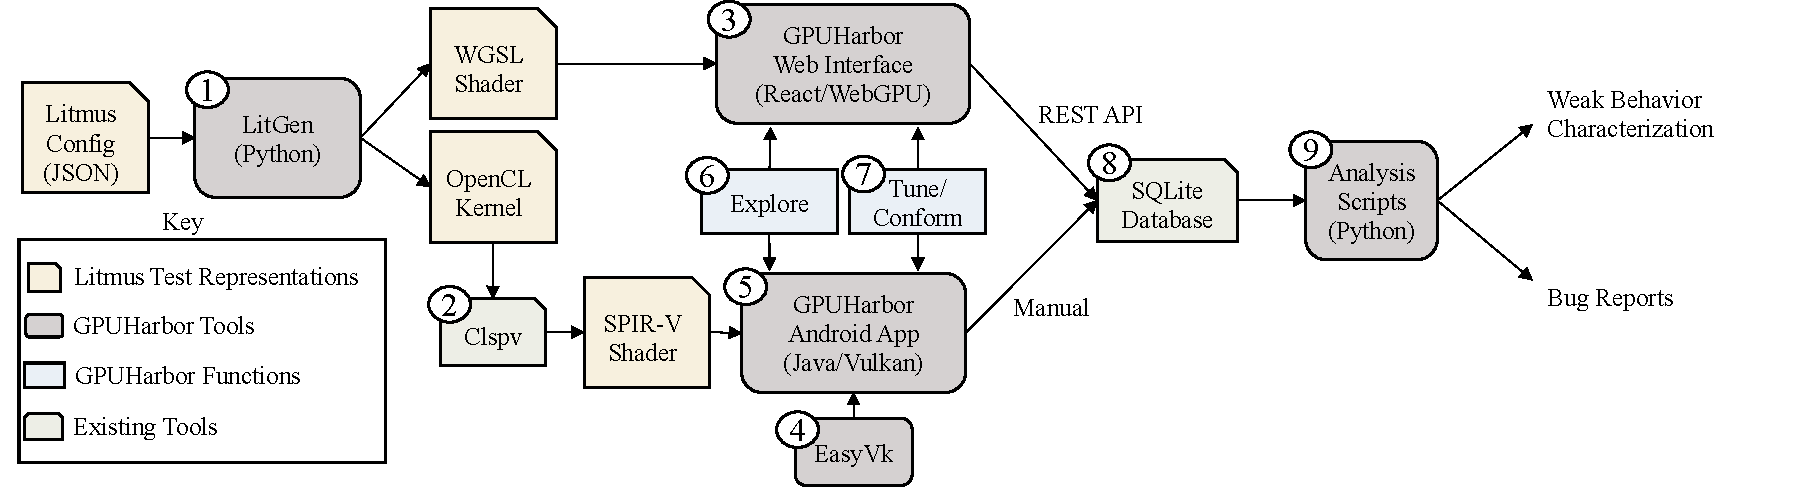
\includegraphics[width=.97\textwidth]{images/system_overview.pdf}
\caption{An overview of the tooling flow for \gpuharbor, with WebGPU and Vulkan MCS targets.}
\label{fig:gpuharbor-sys-overview}
\end{figure*}

\newcommand{\lblitmustest}{
    \begin{tabular}{l l}
    \multicolumn{2}{c}{Initialize: \texttt{x = 0; y = 0;}} \\
    \midrule
    \underline{thread 0} & \underline{thread 1} \\
        \circledBlack{\vphantom{A}a}\hspace{.1cm} \texttt{r0 = L(x);} &  \circledWhite{\vphantom{A}c}\hspace{.1cm} \texttt{r1 = L(y);}  \\
        \circledBlack{\vphantom{A}b}\hspace{.1cm} \texttt{S(y, 1);} &
        \circledWhite{\vphantom{A}d}\hspace{.1cm} \texttt{S(x, 1);}  \\
        \midrule
        \multicolumn{2}{c}{Weak Behavior: \texttt{r0 == 1 \&\& r1 == 1}}

    \end{tabular} \hspace{.5cm}
}

\newcommand{\sblitmustest}{
    \begin{tabular}{l l}
    \multicolumn{2}{c}{Initialize: \texttt{x = 0; y = 0;}} \\
    \midrule
    \underline{thread 0} & \underline{thread 1} \\
        \circledBlack{\vphantom{A}a}\hspace{.1cm} \texttt{S(x, 1);} &  \circledWhite{\vphantom{A}c}\hspace{.1cm} \texttt{S(y, 1);}  \\
        \circledBlack{\vphantom{A}b}\hspace{.1cm} \texttt{r0 = L(y);} &
        \circledWhite{\vphantom{A}d}\hspace{.1cm} \texttt{r1 = L(x);}  \\
        \midrule
        \multicolumn{2}{c}{Weak Behavior: \texttt{r0 == 0 \&\& r1 == 0}}
    \end{tabular} \hspace{.5cm}
}

\newcommand{\storelitmustest}{
    \begin{tabular}{l l}
    \multicolumn{2}{c}{Initialize: \texttt{x = 0; y = 0;}} \\
    \midrule
    \underline{thread 0} & \underline{thread 1} \\
        \circledBlack{\vphantom{A}a}\hspace{.1cm} \texttt{S(x, 2);} &  \circledWhite{\vphantom{A}c}\hspace{.1cm} \texttt{r0 = L(y);}  \\
        \circledBlack{\vphantom{A}b}\hspace{.1cm} \texttt{S(y, 1);} &
        \circledWhite{\vphantom{A}d}\hspace{.1cm} \texttt{S(x, 1);}  \\
        \midrule
        \multicolumn{2}{c}{Weak Behavior: \texttt{r0 == 1 \&\& x == 2}}

    \end{tabular}
}

\newcommand{\readlitmustest}{
    \begin{tabular}{l l}
    \multicolumn{2}{c}{Initialize: \texttt{x = 0; y = 0;}} \\
    \midrule
    \underline{thread 0} & \underline{thread 1} \\
        \circledBlack{\vphantom{A}a}\hspace{.1cm} \texttt{S(x, 1);} &  \circledWhite{\vphantom{A}c}\hspace{.1cm} \texttt{S(y, 2);}  \\
        \circledBlack{\vphantom{A}b}\hspace{.1cm} \texttt{S(y, 1);} &
        \circledWhite{\vphantom{A}d}\hspace{.1cm} \texttt{r0 = L(x);}  \\
        \midrule
        \multicolumn{2}{c}{Weak Behavior: \texttt{r0 == 0 \&\& y == 2}}

    \end{tabular} \hspace{.5cm}
}

\newcommand{\twowritelitmustest}{
    \begin{tabular}{l l}
    \multicolumn{2}{c}{Initialize: \texttt{x = 0; y = 0;}} \\
    \midrule
    \underline{thread 0} & \underline{thread 1} \\
        \circledBlack{\vphantom{A}a}\hspace{.1cm} \texttt{S(x, 2);} &  \circledWhite{\vphantom{A}c}\hspace{.1cm} \texttt{S(y, 2);}  \\
        \circledBlack{\vphantom{A}b}\hspace{.1cm} \texttt{S(y, 1);} &
        \circledWhite{\vphantom{A}d}\hspace{.1cm} \texttt{S(x, 1);}  \\
        \midrule
        \multicolumn{2}{c}{Weak Behavior: \texttt{x == 2 \&\& y == 2}}

    \end{tabular}
}



\begin{figure*}
\centering
\small
\captionsetup[subfigure]{width=.48\textwidth}
\subfloat[Load Buffer (LB)]{\lblitmustest \label{fig:gpuharbor-lb-litmustest}}
\subfloat[Store Buffer (SB)]{\sblitmustest \label{fig:gpuharbor-sb-litmustest}} \\
\subfloat[Store (S)]{\storelitmustest \label{fig:gpuharbor-store-litmustest}}
\subfloat[Read (R)]{\readlitmustest \label{fig:gpuharbor-read-litmustest}} \\
\subfloat[2+2 Write (2+2W)]{\twowritelitmustest \label{fig:gpuharbor-22w-litmustest}} \\
\caption{These litmus tests, along with MP from \myfig\ref{fig:gpuharbor-mp-litmustest}, represent six classic weak behaviors allowed by relaxed MCSs. \texttt{S} and \texttt{L} signify a \texttt{relaxed} atomic store and load, respectively.}
\label{fig:gpuharbor-mcs-litmustests}
\end{figure*}

\section{GPUHarbor System Overview \label{sec:gpuharbor-sys-overview}}

Building on approaches in prior work~\cite{mc-mutants}, we discuss our testing campaign (\mysec\ref{sec:gpuharbor-litmus-selection}) and the development of our MCS testing tools that are easily accessible on a wide range of devices, summarized in \myfig\ref{fig:gpuharbor-sys-overview}. %shows the flow of our tooling for exploring and testing GPU MCSs.
We overview each stage of the tooling, starting with litmus test generation (\mysec\ref{sec:gpuharbor-litmus-test-gen}), moving on to the design of \gpuharbor's web interface and Android app (\mysec\ref{sec:gpuharbor-website-design}). We end the section by describing our data collection process (\mysec\ref{sec:gpuharbor-data-collection}).

\subsection{Litmus Test Selection \label{sec:gpuharbor-litmus-selection}}

The tests we utilize in our study build off of the MCS mutation testing strategy used in~\cite{mc-mutants}. We use 32 \textit{mutants}, out of which 24 are litmus tests with weak behaviors allowed by the WebGPU MCS. The mutants are used to find effective system stress to then run the conformance tests. Our results analysis focuses on characterizing the rates of weak behaviors of six of the mutants, one of which is \textbf{MP} (\myfig\ref{fig:gpuharbor-mp-litmustest}), with the other five shown in ~\myfig\ref{fig:gpuharbor-mcs-litmustests}. These tests enumerate all the combinations of four instructions on two threads that can lead to weak behaviors. Thus, they capture testing for all pair-wise memory reorderings. For example, the \textbf{SB} test checks for store-load reorderings, while the \textbf{LB} test checks for load-store reorderings. Additionally, these tests capture synchronization patterns used in common concurrency algorithms like a compare-and-swap spinlock. Because of this, prior work has also focused on these tests and has shown their utility in finding bugs in both applications and MCS implementations~\cite{gpu-exposing, gpu-foundations}.

%In addition, these six tests represent the core programs used to evaluate MCS testing strategies in~\cite{mc-mutants}, with 24 of the 32 mutants there being either one of the six tests or a slight variation (e.g. adding a memory fence on one thread or changing write values). The other 8 mutants described in that work do not exhibit weak behaviors, only interleaved behaviors, which are not as important to characterize due to the fact that interleaved behaviors are possible under SC and are common on every multi-core architecture.

Once the mutants are run, we use the weak behavior profile of a device to determine an effective system stress configuration to run conformance tests under. We utilize the 20 conformance tests from~\cite{mc-mutants}. As a concrete illustration using one mutant and conformance test, we would run the \textbf{MP} test under many different system stress configurations to build a weak behavior profile. We then use the most effective configuration at revealing \textbf{MP} weak behaviors to run a closely related conformance test, e.g., \textbf{MP-CO} (\myfig\ref{fig:gpuharbor-mp-co-litmustest}). This approach was shown to be effective at finding bugs in prior work~\cite{mc-mutants} and we further show its effectiveness by discovering two new bugs: a violation of \textbf{MP-CO} on Arm devices and a violation of \textbf{MP-CO} on an NVIDIA device (see \mysec\ref{sec:gpuharbor-vulkan-bugs}).
%, one a Mali-G78 GPU in a Google Pixel 6 and the other a Mali-G71 in a Samsung SM-T510, and one in an NVIDIA Tegra X1 in an NVIDIA Shield TV Pro.
%is one such test. Our litmus testing campaigns allow us to find test environments effective at revealing \textbf{MP} weak behaviors at a high rate, and by running \textbf{MP-CO} under these effective test environments we discovered a violation of \textbf{MP-CO} on three devices: two in Arm devices, one a Mali-G78 GPU in a Google Pixel 6 and the other a Mali-G71 in a Samsung SM-T510, and one in an NVIDIA Tegra X1 in an NVIDIA Shield TV Pro.

%The litmus tests in \myfig\ref{fig:gpuharbor-mcs-litmustests} (along with the \textbf{MP} test of \myfig\ref{fig:gpuharbor-mp-litmustest}) are the six litmus tests that we focus on in this study. These tests represent every 2-thread, 4-instruction combination of instructions that can lead to a relaxed behavior. Thus, these tests capture different store and load re-orderings that might happen in a relaxed MCS. Different architectures might allow some or all of these weak behaviors; e.g. only \textbf{SB} is allowed by x86's TSO MCS~\cite{x86-semantics}, while NVIDIA's PTX MCS~\cite{ptx-memory-model} allows all six of the weak behaviors. Both the WebGPU and Vulkan MCSs also allow all of these behaviors, and our goal is to show the rate at which the weak behaviors happen on actual implementations.

%We highlight that these six tests have been the primary focus of prior works~\cite{mc-mutants, gpu-foundations}, due to their simplicity and relative completeness for capturing re-ordering behaviors of loads and stores.

\subsection{Litmus Test Generation \label{sec:gpuharbor-litmus-test-gen}}

We now discuss our tooling that generates and runs our testing and characterization campaign. Litmus test behaviors are non-deterministic and sensitive to system stress. Due to this, the shaders that run the litmus tests contain not only the actual litmus test instructions, like those in \myfig\ref{fig:gpuharbor-mcs-litmustests}, but take in a number of parameters and provide functions that are used to construct system stress.

To provide a standardized interface for defining litmus tests in different GPU languages, we built a tool, Litmus Generator (\textsc{LitGen}, \circledWhite{1} in \myfig\ref{fig:gpuharbor-sys-overview}), which is similar to previous litmus testing tools~\cite{litmus} but is specifically targeted to create GPU programs with system stress, as was shown is necessary for testing GPU MCSs~\cite{gpu-concurrency, gpu-foundations, mc-mutants}. \textsc{LitGen} takes litmus tests that are written in an abstract format, currently JSON, that specify the actions of the test (e.g. loads and stores) and the possible behaviors of the test, with a special designation being given to weak behaviors. The tests used in this work were all manually specified, as they are relatively small, but \textsc{LitGen} could be integrated with other tools that use formal models to generate litmus tests, e.g., ~\cite{fences, memalloy}, which would provide more automation and account for more complicated tests and MCSs. \textsc{LitGen} outputs a \textit{test shader}, which runs the test alongside system stress developed in prior work~\cite{mc-mutants, gpu-foundations}, and a \textit{result shader}, which aggregates the observed behaviors of the test.

The result shader is generated separately from the test shader for several reasons:
\begin{enumerate}
    \item Some tests, like \textbf{2+2W} (\myfig\ref{fig:gpuharbor-22w-litmustest}), examine memory locations for weak behaviors after all threads have finished executing the test. To avoid relying on synchronization features (some of which we are trying to test), we instead pass the test memory buffer into a new result aggregation shader, which executes after the test shader.
    \item \textsc{LitGen} implements parallel testing, described in~\cite{mc-mutants}, which runs thousands of \textit{instances} of each litmus test concurrently. Thus, it is natural to leverage the inherent parallelism of the GPU to also aggregate the many results, which otherwise may be time-consuming to do on the CPU, especially since it requires copying memory from the GPU to the CPU.
\end{enumerate}

Currently, two backends exist for \textsc{LitGen}. The tool outputs WGSL shaders directly, as WGSL is a text-based language. SPIR-V, on the other hand, is a low-level representation similar to LLVM, increasing its flexibility but making code generation more complex. Therefore, for Vulkan backends \textsc{LitGen} first outputs OpenCL, a compute-focused GPU language, which is similar in syntax to C++. Then, it utilizes Clspv~\cite{clspv} (\circledWhite{2}), a prototype compiler from OpenCL to SPIR-V, to generate the shader used in the Android app.

As WebGPU is primarily browser-based while Vulkan runs on native devices, we currently maintain litmus testing driver programs in two languages. WebGPU exposes a relatively simple JavaScript API, on which we build our web interface (\circledWhite{3}). %In this interface, we include features that increase the system stress, such as passing buffers to the shader that map built-in thread and workgroup identifiers to a new, randomized identifier.
%
Vulkan's native C/C++ API is more complex, so to simplify this process, we have built a Vulkan compute wrapper which we call \textsc{EasyVk} (\circledWhite{4}). This library exposes a simple interface where buffers are defined and shaders dispatched to the GPU in a few lines of code. \textsc{EasyVk} is integrated into the Android app and included as part of our artifact.

\subsection{\gpuharbor Design \label{sec:gpuharbor-website-design}}

\begin{figure}
\hfill
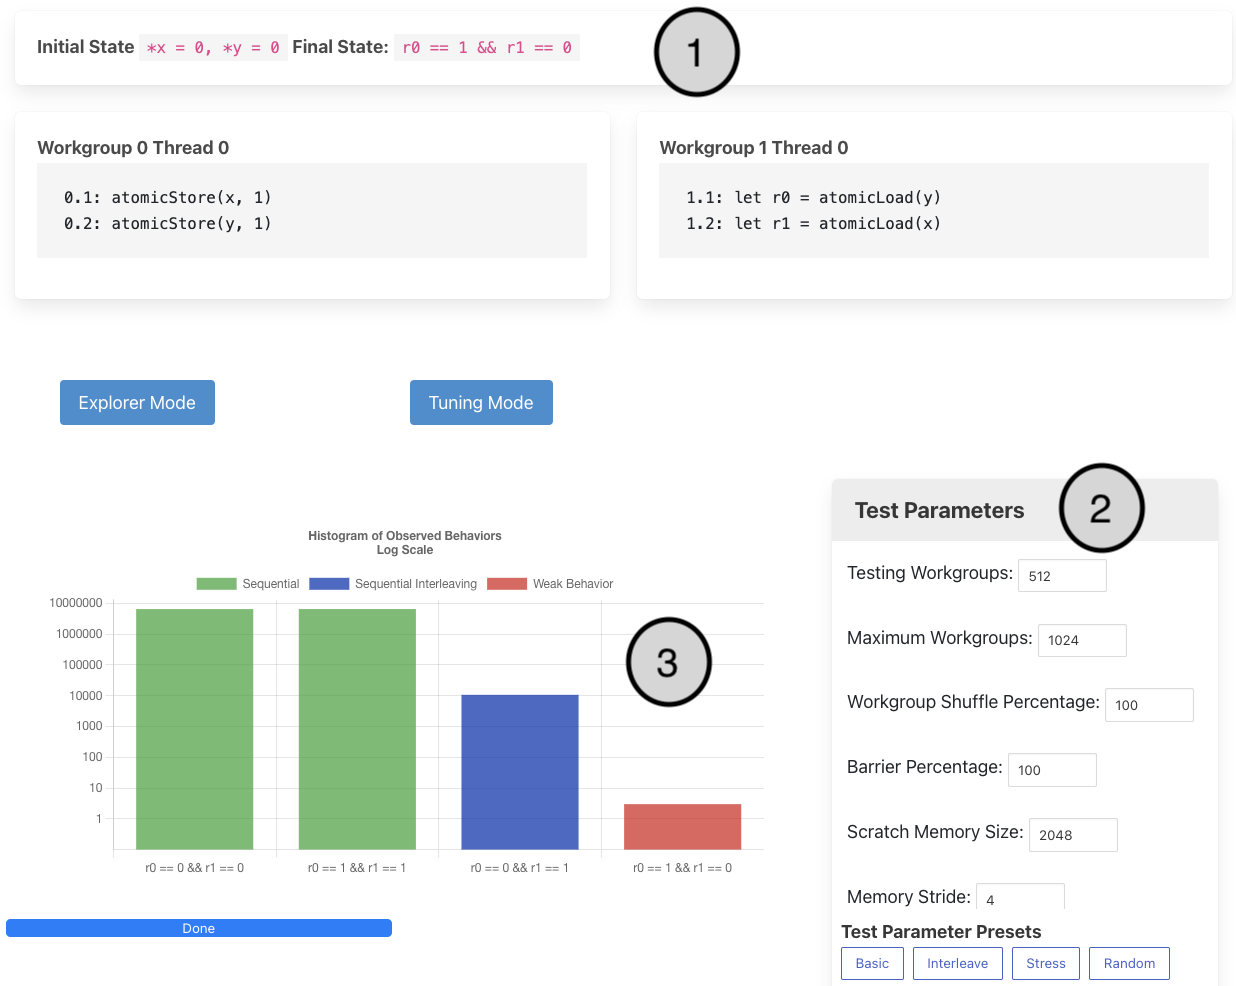
\includegraphics[width=\columnwidth]{images/gpuharbor.png}
\caption{A screenshot of \gpuharbor's web interface showing the ``Explore'' page for the \textbf{MP} litmus test.}
\label{fig:gpuharbor-interface}
\end{figure}

Previous GPU MCS studies have been limited in reach due to the difficulty in deploying cross-platform GPU applications~\cite{opencl-hitchhiker}. One of the reasons for this is the fractured landscape of GPU development. NVIDIA's popular CUDA framework~\cite{cuda} is used for many data science applications but is only supported on NVIDIA GPUs. OpenCL~\cite{opencl} was introduced in 2009 by Apple as a cross-platform standard; however, today Apple no longer supports OpenCL and instead requires developers to use their proprietary Metal API~\cite{metal}. %and the future of OpenCL remains unclear.

Another issue with previous GPU MCS testing approaches has been a reliance on expert users to run testing campaigns. For example, using OpenCL would require users to install the required drivers, build the application under a specific environment, etc. To collect data from the diversity of devices necessary to gain confidence in cross-platform GPU frameworks, tools must minimize the friction in setting up and running tests. The tools we introduce here are easily distributed applications with a user-friendly interface on top of new GPU frameworks so that even non-technical users can collect data on their devices and submit results for analysis. To this end, we introduce \gpuharbor: a GPU MCS testing tool with two widely supported and accessible frontends, a web interface and an Android app (\circledWhite{3} and \circledWhite{5} in \myfig\ref{fig:gpuharbor-sys-overview}).

\gpuharbor's web interface and Android app have a common design with two functions: exploring (\circledWhite{6}) and tuning/conforming (\circledWhite{7}). ``Explore'' pages run specific litmus tests, display histograms of results, and provide the ability to adjust various parameters that control system stress. When tuning and conforming, a set of tests are chosen to run with multiple random system stress configurations, searching for configurations that maximize the rate of weak behaviors and uncover bugs in MCS implementations. While this study includes the largest collection of data on mobile GPU MCS behaviors, in \mysec\ref{sec:fut-work} we discuss future work that could increase the reach of mobile GPU MCS testing even further.

\paragraph{Exploring\label{sec:gpuharbor-sys-overview-explore}}

\myfiglong\ref{fig:gpuharbor-interface} shows a screenshot of \gpuharbor's web interface explore page for the \textbf{MP} litmus test after the test has been run with relatively high systems stress on a MacBook Pro with an integrated Intel Iris GPU. The top of the page (\circledGrey{1}) includes a description of the test and pseudocode showing the test instructions. The right-hand side (\circledGrey{2}) includes an editable list of the parameters that define system stress, along with several presets. When the test is running, the histogram (\circledGrey{3}) updates in real-time with the number of times each behavior is observed. The progress bar gives an estimate of how much longer is left to run, based on the speed of previous iterations.

The green bars correspond to sequential behaviors, where one thread runs entirely before the other. The blue bar corresponds to interleaved behaviors, where actions from each thread are interleaved (e.g. leading to the behavior \texttt{r0 == 0 \&\& r1 == 1} in the \textbf{MP} litmus test). The red bar corresponds to weak behaviors; in this run, three \textbf{MP} weak behaviors were observed out of over 13 million test instances, so the histogram shows behaviors (using a log scale, as weak behaviors are relatively rare).

%We have found that test exploration is useful in several ways. When designing experiments, we can quickly iterate on different system stress configurations and number of iterations. It has also proved useful as a pedagogical tool for teaching both GPU programming and the weak behaviors allowed by relaxed MCSs, which we expand on in \mysec\ref{sec:gpuharbor-eval-ped}.

\paragraph{Tuning and Conforming\label{sec:gpuharbor-sys-overview-tune-conform}}

Both the web interface and the Android app can be used to tune system stress, as in~\cite{mc-mutants}. When tuning, a set of tests can be selected, with presets available for weak memory tests (e.g. those in \myfig\ref{fig:gpuharbor-mcs-litmustests}) and conformance tests, e.g., to test coherence.
%(e.g. if the memory orders of the tests in \myfig\ref{fig:gpuharbor-mcs-litmustests} are strengthened to disallow the weak behavior).
Testing options like the number of configurations, the maximum number of workgroups, and other parameter overrides can be modified to run different experiments and check specific tests without redeploying any code.

To collect data from volunteer users across a diverse set of devices, we strive to minimize the options users have to configure. This reduces the chances of errors and provides us with a standardized dataset to analyze. The web interface's tuning page, therefore, includes a tab that exposes no configuration options, but instead shows only a few buttons: one button that starts a combined tuning/conformance run with default parameters: and another button that pulls up a submission form, which submits the results along with some (optional) contact information. Our results are all anonymized; contact details were only collected if users wanted to be informed about the outcome of the study. Before submitting, users agreed that their anonymized results could be aggregated, reported on, and released as part of this study.
%We detail this setup and data collection process in the next section.

\subsection{Data Collection \label{sec:gpuharbor-data-collection}}

To submit test data, the web interface communicates with a backend service that exposes an API for submitting results and inserting them into an SQLite database (\circledWhite{8} in \myfig\ref{fig:gpuharbor-sys-overview}). %After completing a test run, users can pull up a form where contact and system information can be filled out before confirming they wish to send the results to us,
The data is then analyzed using Python scripts (\circledWhite{9}).
%
The Android app is not yet available on the app store nor is it integrated with the SQLite backend, so results are manually copied off of the device for analysis. In \mysec\ref{sec:fut-work} we discuss how we can reduce the friction for submitting mobile app results, and thus, increase the reach of future studies.  Nevertheless, our study of eight devices is the largest testing campaign of mobile GPU MCS behaviors of which we are aware.

While system stress configurations are generated randomly, we would like to ensure that the configurations run on different devices are the same for data analysis purposes. That is, if different GPUs are tested with the same stress configurations, we can compare how the different devices behaved under the same stress. We ensure this by integrating a seedable Park-Miller random number generator~\cite{prng} into both the web interface and the Android app and using the same seed when running all of our tuning experiments.

By default, browsers only expose limited information about the user's GPU without turning on vendor-specific development flags due to privacy and security concerns around fingerprinting~\cite{webgpu-security}. In order to have as much information as possible about our data, we included instructions asking users to temporarily enable flags so we could collect detailed GPU information. Of the 98 results we collected, 67 included the exact GPU tested. The other 31 results did not specify the exact GPU, but included only the vendor and a string describing the GPU architecture, such as ``intel gen-9'' or ``nvidia ampere''. All Apple devices reported an architecture of ``common-3'', making it impossible to immediately distinguish M1's vs M2's. However, we show in \mysec\ref{sec:gpuharbor-webgpu-sim} that our data can be used to infer device information, hindering the ability of browsers to hide the specifics of a user's GPU.




%The goals of our experiment are both to reveal weak behavior rates and to run conformance tests. As mentioned in \mysec\ref{sec:litmus-testing}, we draw from the mutation approach described in~\cite{mc-mutants} and include the 32 mutants defined in that paper as our tuning tests.
%The tests include the six classic weak memory litmus tests shown in ~\myfig\ref{fig:gpuharbor-mcs-litmustests} as well as variants that strengthen some memory accesses to an acquire or release memory order using memory fences or change atomic loads/stores into atomic RMWs.

%The 32 mutants are run for a set number of configurations and iterations, with the test framework keeping track of the environment that maximizes the rate of weak behaviors per test. Once the tuning run is complete, the best test environment per mutant is used to run one of 20 conformance tests in order to search for bugs without also having to tune over the conformance tests themselves. All of these results are then structured via JSON recording the number of behaviors, test environment parameters, and device/platform information and can be submitted for analysis.

\section{Initial Results: Weak Behavior Characterization \label{sec:gpuharbor-wb-char}}

\begin{figure}
\hfill
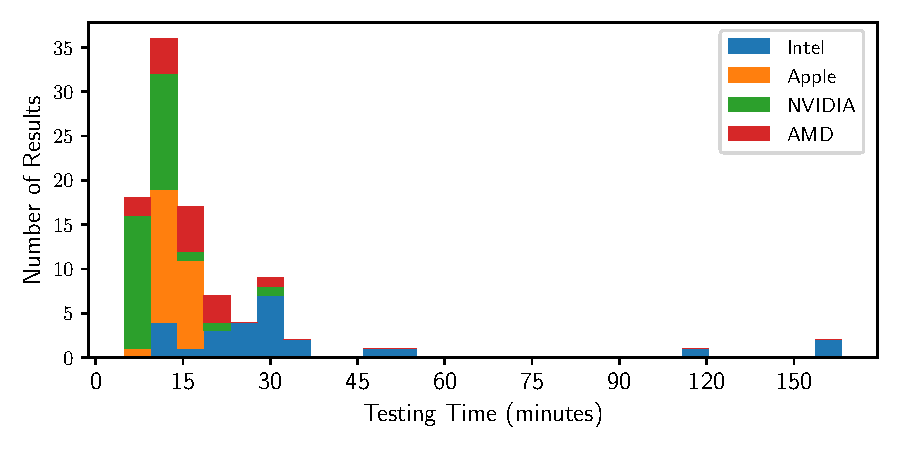
\includegraphics[width=\columnwidth]{images/webgpu-timing.pdf}
\caption{Histogram showing the time spent testing WebGPU's MCS on each device using \gpuharbor's web interface. Each bin is broken down by vendor.}
\label{fig:gpuharbor-webgpu-timing}
\end{figure}

To collect data from as many sources as possible, we disseminated the link to \gpuharbor's web interface to the general public, utilizing campus forums and social media, and ran the Android app on eight devices that we could physically access. As shown in \mytab\ref{tab:gpuharbor-gpu-overview}, we collected data from millions of tests; each test used a randomly generated system stress configuration (we used 50 configurations on the web interface and 150 on the Android app). In each configuration, tests were run millions of times based on a randomly generated number of workgroups and threads per workgroup.

To ensure data integrity, we implemented a checksum algorithm that verified we saw the expected number of overall behaviors based on the system stress configuration. The testing duration was also recorded, however, we ran into one issue here. Some computers went to sleep in the middle of the tests, suspending the browser's process and leading to extremely long recorded test times. To overcome this, we recorded testing time on a per test/configuration basis; we then filtered the results so as to not include any test/configuration durations over one minute. We note that each individual test runs quickly (e.g. in less than 5 seconds), thus, runs that were over one minute were most likely when the computer went to sleep. To approximate the length of the test that was suspended, we used a neighboring test's time.

%We found that mobile GPUs were much more limited in their capacity; for example, in our WebGPU study we ran up to 1024 workgroups with 256 threads per workgroup, but depending on the Android device, we had to limit the number of workgroups and workgroup sizes to between 8 and 32.

One consideration for collecting data from the wider public is that we cannot afford to run tests for hours at a time. Previous work targeted only a few devices, running tests on one device for a minimum of 36 hours~\cite{gpu-foundations} or 2 hours~\cite{mc-mutants}. However, asking volunteer users to leave their browsers and computer open for that long is impractical and would certainly decrease the number of submissions. Therefore, we heuristically chose the number of test environments and iterations per environment, aiming for the tests to finish in 10-20 minutes.

\myfiglong\ref{fig:gpuharbor-webgpu-timing} shows the distribution of testing time on our web interface, broken down by vendor. The results show that NVIDIA devices were the fastest on average, mostly running all tests in under 15 minutes. On the other hand, Intel devices ran slower, with two older Intel GPUs taking over an hour and a half to complete. %Due to a recording error, we do not have accurate timing information on the experiments run on the Android app, but we do know that each device took at least one hour, and we plan on re-running our experiments to collect accurate timing data.

In the rest of this section, we analyze our WebGPU and Vulkan data to characterize the rates at which weak behaviors occur on devices from different vendors. These initial results motivate three research questions, which are explored in depth in \mysec\ref{sec:gpuharbor-insight-impact}:

\begin{enumerate}
    \item Do MCS bugs exist in the wild, especially in GPUs which are relatively untested (\mysec\ref{sec:gpuharbor-vulkan-bugs})?
    \item Can our characterization data  be used to identify similarities between GPUs (\mysec\ref{sec:gpuharbor-webgpu-sim})? If so, then our data can be used to develop new testing strategies or to expose potential new browser fingerprinting vulnerabilities.
    \item How can a weak behavior characterization study be used in programming guides for implementing synchronization constructs, e.g. mutexes (\mysec\ref{sec:gpuharbor-vulkan-locks})?
\end{enumerate}

\subsection{Weak Behaviors in WebGPU \label{sec:gpuharbor-webgpu-eval-weak}}

\begin{figure}
\hfill
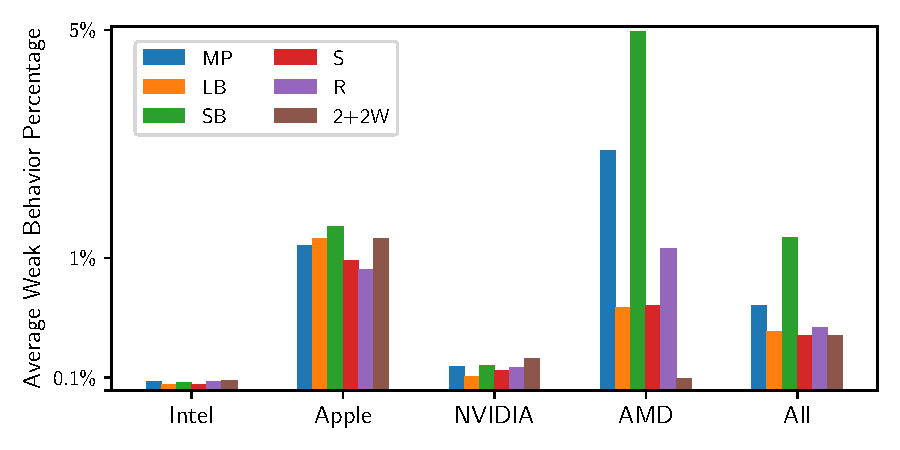
\includegraphics[width=\columnwidth]{images/webgpu-rates.pdf}
\caption{Data showing the average rate of weak behaviors across vendors when running litmus tests using WebGPU.}
\label{fig:gpuharbor-webgpu-rates}
\end{figure}

%\begin{figure}
%\hfill
%\includegraphics[width=\columnwidth]{images/webgpu-medians.pdf}
%\caption{Data showing the median rate of weak behaviors across vendors when running litmus tests using WebGPU.}
%\label{fig:gpuharbor-webgpu-medians}
%\end{figure}

\myfiglong\ref{fig:gpuharbor-webgpu-rates} shows the average rates of observed weak behaviors for the six litmus tests of \myfig\ref{fig:gpuharbor-mcs-litmustests} (plus \textbf{MP}) in the test environment that maximizes the rate on each device broken down by test and vendor. As described in \myfig\ref{tab:gpuharbor-gpu-overview}, we have data from at least 15 devices from each vendor. The overall testing time across all \webGPUDevices devices was 31.1 hours, an average of 19 minutes per device. %The distribution of testing time on each device is shown in \myfig\ref{fig:gpuharbor-webgpu-timing}; the two outliers that took over an hour and a half were both older Intel GPUs.

Devices from all vendors showed weak behaviors on each litmus test. In all but two cases, observing weak behaviors was all or nothing; if a device revealed weak behaviors on one litmus test, it revealed weak behaviors on all of them. In contrast, on a device implementing x86's TSO MCS, we would expect to only see store buffering behaviors. However, unlike x86, GPU devices do not provide low-level details, such as the hardware-level MCS, thus it was not clear what types of weak behaviors we would observe. These results show that many GPUs implement very relaxed memory models, in contrast to stronger CPU architectures like x86 TSO.

Intel devices tended to have the lowest rate of weak behaviors, with just over half of them (15/26) revealing weak behaviors on each test. The median rate of weak behaviors on Intel devices was even lower than their average, around .02\% for each test. No Intel device showed a rate of weak behaviors above 1\% on any test.

NVIDIA devices revealed weak behaviors at a relatively low rate. Our results include results from NVIDIA's Kepler (2012), Maxwell (2014), Pascal (2016), Turing (2018), and Ampere (2020) architectures, with a majority being the more recent Ampere. Older devices generally showed fewer weak behaviors, with the minimum on each of the six tests being Kepler and Maxwell devices. However, one outlier is that the maximum rate of \textbf{SB} behaviors (.73\%) was seen on a Kepler device. Interestingly, that device was also the only device not to observe any weak behaviors on \textbf{S}, \textbf{LB}, and \textbf{2+2W}. The only other device not to reveal weak behaviors on a test was a Quadro K620 with a Maxwell architecture, on \textbf{MP}, \textbf{R}, and \textbf{SB}.

Apple devices were consistently weak, revealing weak behaviors on every device and test, generally at a higher rate on all tests than NVIDIA devices but with less variation than AMD devices. Apple GPUs have only been recently built into non-mobile devices, so these results represent the first comprehensive evaluation of the weak behaviors on Apple GPUs. We don't have the specific name of every Apple device, but we were able to collect enough information to show we had results from Apple M1 (basic, Pro, Max) and Apple M2 (basic, Pro) devices.

AMD devices were also very weak, with 100\% of devices showing weak behaviors on every test. The clear highest average rate occurs on the \textbf{SB} litmus test on AMD GPUs. Most of the AMD devices show a high rate of weak behaviors on \textbf{SB}, approaching 10\% and higher, but devices with AMD's Graphics Core Next 5 micro-architecture all showed rates under 1\%. This means that even from a single vendor, the behaviors of different architectures can vary widely and past results from one vendor cannot be counted on to predict future behaviors.

\subsection{Weak Behaviors in Vulkan \label{sec:gpuharbor-vulkan-weak}}

\begin{table}
\footnotesize
\centering
\caption{Data showing the average rate of weak behaviors across vendors when running litmus tests using Vulkan.}
\scalebox{0.95}{\begin{tabularx}{1.02\columnwidth}{ l l r r r r r r }
 \toprule
 & & \multicolumn{6}{c}{\textbf{Litmus Test}} \\
\cmidrule(lr){3-8}
\textbf{Vendor} & \textbf{Device} & \textbf{MP} & \textbf{LB} & \textbf{SB} & \textbf{S} & \textbf{R} & \textbf{2+2W} \\
\midrule
\multirow{4}{*}{Qualcomm} & Adreno 610 & 0\% & 0\% & 0\% & 0\% & 0\% & 0\% \\
& Adreno 640 & 0\% & 2.04\% & 1.45\% & 1.65\% & 0\% & 2.21\% \\
& Adreno 642L & 0.04\% & 5.75\% & 5.81\% & 3.81\% & 0\% & 6.38\% \\
& Adreno 660 & 0.12\% & 8.5\% & 14.37\% & 5.69\% & 0\% & 11.5\% \\
\midrule
\multirow{2}{*}{Arm} & Mali-G71 & 0.04\% & 0\% & 0\% & 0\% & 0\% & 0\% \\
& Mali-G78 & 1.56\% & 0\% & 0\% & 0\% & 0\% & 0\% \\
\midrule
Imagination & PowerVR  & 0\% & 0\% & 0\% & 0\% & 0\% & 0\% \\
& GE8320 & & & & & & \\
\midrule
NVIDIA & Tegra X1 & 0.01\% & 0.05\% & 0.02\% & 0.01\% & 0.01\% & 0.05\% \\
 \bottomrule
\end{tabularx}}
\label{tab:gpuharbor-vulkan-rates}
\end{table}

The data in \mytab\ref{tab:gpuharbor-vulkan-rates} shows the percentage of weak behaviors in the test environment that maximizes the rate at which they occur for our Android devices. In contrast to our web GPUs, in the mobile setting, weak behaviors were observed in every test on only one device, the NVIDIA Tegra X1, but the rates on this device were very low, beneath 0.1\%. The most difficult test to observe in general was \textbf{R}, which checks whether a store is reordered with a following load on one thread. We did not observe any weak behaviors on the Imagination GPU; because testing is fundamentally incomplete, this could mean that the device implements a strong MCS, or that our testing approach was not effective. Interestingly, ARM only showed weak behaviors in the \textbf{MP} test.

We observe that, in general, the rates of weak behaviors increase as devices become more powerful. This is especially apparent from the four Qualcomm devices we test, as the rate of weak behaviors increases from 0\% on the Adreno 610 (which has 96 \textit{shading units}, analogous to NVIDIA's CUDA cores) up to a maximum of 14.37\% in \textbf{SB} on the Adreno 660 (with 512 shading units). One intuitive explanation for this might be that smaller GPUs lack the ability to schedule as many threads at once, naturally reducing the rates of weak behaviors despite architectures that might allow them. We see a similar trend on the Arm GPUs, where the smaller Mali-G71 (32 shading units) showed a lower rate of weak behaviors than the larger Mali-G78 (384 shading units).

%Similar to the WebGPU study, the takeaway from these results is that applications should be tested on a variety of devices for conformance. Instead of choosing one GPU from Qualcomm and one from Imagination, it may be a better idea to choose devices from different behavior classes, such as a Qualcomm 610 and a Qualcomm 660.

\section{Insights and Impacts \label{sec:gpuharbor-insight-impact}}

We now set out to answer the three questions posed in \mysec\ref{sec:gpuharbor-wb-char} using our data and characterization of weak behavior rates.

\subsection{MCS Bugs \label{sec:gpuharbor-vulkan-bugs}}

Our conformance testing campaigns discovered bugs on several vendors' devices when running under the Vulkan and WebGPU frameworks.

\begin{enumerate}
    \item \textbf{Arm}: We observed coherency violations of the \textbf{MP-CO} litmus test when using the Vulkan framework on two Arm GPUs, a Mali-G71 and a Mali-G78. These bugs were reported to and confirmed by Arm, leading to a compiler fix to insert a missing memory fence. Arm has also added regression tests based on the pattern of the violation we reported.
    \item \textbf{NVIDIA}: We also observed violations of the \textbf{MP-CO} test when run using the Vulkan framework on an NVIDIA Tegra X1.  Additionally, our WebGPU conformance test results revealed violations of a different coherence test, \textbf{RR}, on an NVIDIA Quadro P620 running on a Linux desktop (therefore using Vulkan as the native framework). The combined report of the bug on the Tegra X1 and Quadro P620 helped NVIDIA find and fix a bug in their Vulkan compiler. NVIDIA also noted that this bug affected the Vulkan compiler in all pre-Volta architecture GPUs.
    \item \textbf{Apple}: Our WebGPU conformance tests reveal coherence violations in \textbf{RR} from eight other devices, all running on Apple machines. Five of these devices were Intel GPUs, two were NVIDIA GPUs, and one was an AMD GPU.  MCMutants observed the same issue on an Intel integrated device on a MacBook and reported the issue to Apple~\cite{mc-mutants}; the bug has not been confirmed nor fixed.  On Intel, it is likely that these bugs are instances of the same issue, but our results are the first time the bug has been observed on non-Intel GPUs.
\end{enumerate}

We found all of the bugs by running conformance litmus tests under tuned system stress. We choose the system stress using the methodology described in prior work~\cite{mc-mutants}, i.e., by selecting a system stress configuration effective at revealing weak behaviors in an associated weak memory litmus test. For the \textbf{MP-CO} bugs on the Arm and NVIDIA devices, we perform a correlation analysis to empirically validate the methodology.

We run both the \textbf{MP} and \textbf{MP-CO} litmus tests in 150 randomly generated system stress configurations on each of the Android devices showing the bug, recording the rate of weak behaviors in \textbf{MP} and the rate of buggy (i.e. non-coherent) behaviors in \textbf{MP-CO}. Our results show that the Pearson Correlation Coefficient (PCC) between the rate of weak and buggy behaviors is 0.732 on the Arm Mali-G71, 0.759 on the Arm Mali-G78, and 0.832 on the NVIDIA Tegra X1. Since these behaviors are recorded from 150 samples (i.e. system stress configurations), we have 148 degrees of freedom, and running a Student's t-test leads to a p-value less than $10^{-5}$\% on each device. This shows that the PCC between weak behaviors and bugs is certainly not due to random chance, further validating that configurations tuned using weak behaviors are effective at revealing bugs in conformance tests.

%\subsection{WebGPU Inter-Workgroup Synchronization \label{sec:gpuharbor-webgpu-conform}}

%\begin{figure}
%\hfill
%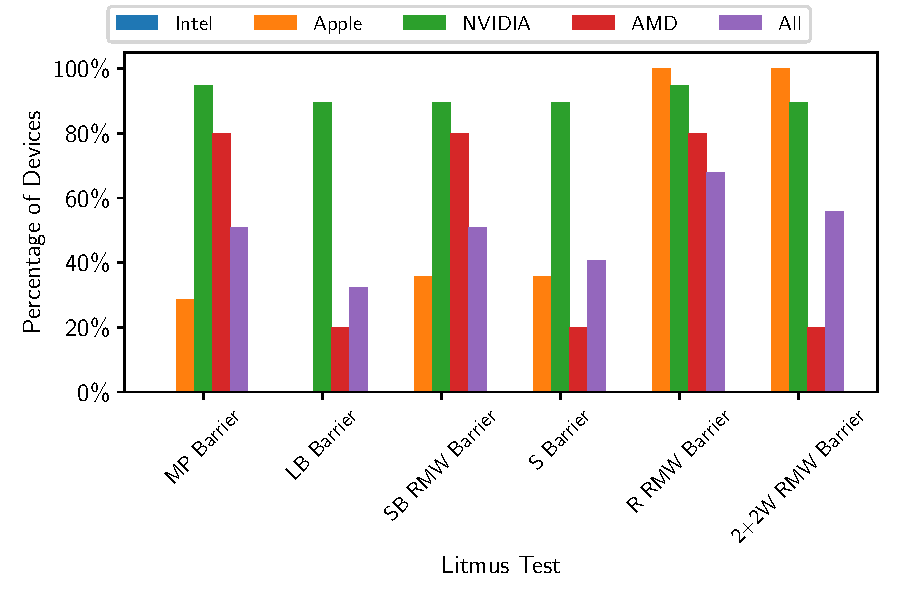
\includegraphics[width=\columnwidth]{images/webgpu-conformance.pdf}
%\caption{The percentage of devices per vendor that show weak behaviors in WebGPU with barriers inserted.}
%\label{fig:gpuharbor-webgpu-conformance}
%\end{figure}

%\myfiglong\ref{fig:gpuharbor-webgpu-conformance} shows the percentage of devices where a weak behavior is observed even with a \texttt{storageBarrier} inserted between instructions in different litmus tests. Three of the six tests are RMW variants, as some instructions in these tests need to be modified to be an RMW to introduce synchronization with an acquire/release memory order.

%The data indicates that on devices from many vendors, weak behaviors still occur even with barriers inserted. As noted in \mysec\ref{sec:background-gpu}, earlier versions of the WebGPU specification disallowed these behaviors, but since that change, it is likely that compilers have changed to not try and enforce inter-workgroup synchronization when a \texttt{storageBarrier} is used. Specifically, the NVIDIA PTX memory model is known to implement inter-workgroup acquire and release fences, so the fact that all six weak behaviors are observed on all NVIDIA devices is indicative the fences are not being inserted.

%Despite this, no weak behaviors are observed on any Intel devices in tests with barriers. In \myfig\ref{fig:gpuharbor-webgpu-rates}, we showed that Intel had the lowest average rate of weak behaviors on all tests, but if compilers were not implementing the \texttt{storageBarrier} as an inter-workgroup acquire/release fence, we might still expect to see some weak behaviors. This means that an algorithm requiring inter-workgroup synchronization implemented in WebGPU and tested on an Intel device may run correctly, leading to the incorrect conclusion that the algorithm will behave as expected on other devices.

%These results show that the tools we introduce will be an important source of data if WebGPU decides to support inter-workgroup synchronization, testing compiler changes and many implementations for conformance to new specifications.

\subsection{GPU Similarity \label{sec:gpuharbor-webgpu-sim}}

\begin{table}
\centering
\caption{Each row shows the cosine similarity statistics between all pairs of devices from that vendor. The last row shows the similarity statistics across all pairs of devices.}
\begin{tabularx}{\columnwidth}{X Y Y Y Y }
\toprule
\textbf{Vendor} & \textbf{Avg} & \textbf{Median} & \textbf{Min} & \textbf{Max} \\
\midrule
Intel & 0.870 & 0.891 & 0.683 & 0.985 \\
Apple & 0.903 & 0.913 & 0.699 & 0.993 \\
NVIDIA & 0.903 & 0.931 & 0.670 & 0.996 \\
AMD & 0.904 & 0.927 & 0.661 & 0.989 \\ \hline
All & 0.840 & 0.862 & 0.477 & 0.996 \\
\bottomrule
\end{tabularx}
\label{tab:gpuharbor-webgpu-sim-stats}
\end{table}

\begin{table}
\centering
\caption{Device clustering shows that choosing one device from each vendor is not an optimal way to test applications that utilize the MCS.}
\begin{tabularx}{.7\columnwidth}{ X r r r r r r }
\toprule
& \multicolumn{6}{c}{\textbf{Cluster}} \\
\cmidrule(lr){2-7}
\textbf{Device} & \textbf{A} & \textbf{B} & \textbf{C} & \textbf{D} & \textbf{E} & \textbf{F} \\
\midrule
Intel & 3 & 0 & 0 & 5 & 18 & 0 \\
Apple & 12 & 4 & 0 & 10 & 0 & 0 \\
NVIDIA & 1 & 0 & 19 & 8 & 2 & 1 \\
AMD & 13 & 1 & 0 & 1 & 0 & 0 \\
\bottomrule
\end{tabularx}
\label{tab:gpuharbor-webgpu-clusters}
\end{table}

All of the data was collected by running the tests with pseudo-randomly generated system stress configurations, but as mentioned in \mysec\ref{sec:gpuharbor-data-collection} the generator is seeded with a known value. Thus, we can compare how different GPUs behave under the same stress parameters. To do this, each testing run is represented as a vector of the non-sequential (i.e. where one thread runs entirely before another one) behaviors of every test in each configuration. Ignoring the sequential behaviors gives the data a degree of freedom, which is necessary for calculating a valid similarity measure.

For our similarity metric, we choose \textit{cosine similarity}, which measures the cosine of the angle between two vectors and ranges from -1 to 1. We chose cosine similarity because it is a relative metric, not an absolute like Euclidean distance, meaning that devices that show different absolute rates of behaviors, but at similar relativity, are classified as more closely related.

 \paragraph{Device Identification} \mytablong\ref{tab:gpuharbor-webgpu-sim-stats} shows a summary of the similarity between devices in our study. All similarities are positive, with the minimum being 0.477 between an Intel and AMD device. This is not surprising, since effective system stress is likely to reveal weak behaviors on many devices. However, the average and median similarities between devices from each vendor are higher than the overall average and median, showing that in general devices from the same vendor tend to have more similar MCS behaviors.

 For Apple and NVIDIA, we confirmed that the maximum similarity occurs between identical GPUs: two Apple M1 Max's and two NVIDIA GeForce RTX 3080s. For AMD, we observe a maximum similarity of 0.989 between two devices, one of which is a Radeon Pro 5500M (\textbf{A}) while the other device (\textbf{B}) did not report a model and instead only indicated that it was from the same architectural generation as \textbf{A}. However, we observed a high similarity (0.985) between \textbf{A} and another Radeon Pro 5500M (\textbf{C}), as well as a similarity of 0.984 between \textbf{B} and \textbf{C}, so it seems likely that \textbf{A}, \textbf{B}, and \textbf{C} are all the same device. We do a similar analysis with Intel to determine that an unknown device is most likely an Intel Iris Xe Graphics. While we are most interested in using this data to help choose conformance test strategies, as shown next, we also note that GPU MCS behavior data like this exposes a fingerprinting vulnerability, despite the specification trying to hide specific device information for security reasons.

%Other research has shown how GPU performance data can be used as a fingerprint~\cite{gpu-fingerprint}

\paragraph{Clustering Based Testing Strategies} K-means clustering attempts to minimize the \textit{distortion}, or the sum of squared distances between vectors and a centroid. Applying k-means clustering to GPU MCS behavior has implications for testing strategies; when developing cross-platform GPU applications that rely on shared memory operations, testing these applications on a number of devices can increase confidence in the correctness of the implementation. A naive strategy might be to choose one device from each major vendor, but our results show that this is not necessarily an optimal strategy.

\mytablong\ref{tab:gpuharbor-webgpu-clusters} shows the result of running k-means with six clusters on the similarity data from \mytab\ref{tab:gpuharbor-webgpu-sim-stats}. The ``elbow-method'' heuristic showed that the rate of decrease in distortion leveled off at 6 clusters on our data. The clustering data shows that devices from the same vendor are generally placed into the same cluster, but there are outliers in each case. The only NVIDIA Kepler device in our study was dissimilar enough from other devices that it was placed in its own cluster. Kepler is also the oldest NVIDIA architecture in our study, showing that special testing attention might be needed when supporting older devices in cross-platform GPU frameworks.

When selecting which devices to test a shared memory GPU application on, the strategy should be to first choose a number of clusters based on the rate of decrease in distortion, and then select at least one device from each cluster. Using our data, this might mean selecting an AMD device from \textbf{A}, Apple devices from clusters \textbf{B} and \textbf{D}, NVIDIA devices from clusters \textbf{C} and \textbf{F} (the only device in that cluster), and an Intel device from cluster \textbf{E}. Despite choosing more Apple and NVIDIA devices than AMD and Intel, the similarity data ensures the tests maximally cover devices with different behavior profiles.

\subsection{Implementing Synchronization Algorithms \label{sec:gpuharbor-vulkan-locks}}

\begin{table}
        \centering
        \caption{Analysis of three locking algorithms, Test-and-Set (TAS), Test and Test-and-Set (TTAS), and Compare-and-Swap (CAS), showing in how many test runs (out of 1000) we observed failures of unfenced (UF) and fenced (F) lock implementations to protect a critical section. The total time to run all tests on each device is also recorded.}
        \begin{tabular}{ l r r r r r r r }
        \toprule
        & & \multicolumn{2}{c}{\textbf{TAS}} & \multicolumn{2}{c}{\textbf{TTAS}} & \multicolumn{2}{c}{\textbf{CAS}} \\
        \cmidrule(lr){3-4} \cmidrule(lr){5-6} \cmidrule(lr){7-8}
        \textbf{Device} & \textbf{Time (min)} & \textbf{UF} & \textbf{F} & \textbf{UF} & \textbf{F} & \textbf{UF} & \textbf{F} \\
        \midrule
         Adreno 610 & 3.5 & 0 & 0 & 0 & 0 & 0 & 0 \\
         Mali-G78 & 67.9 & 18 & 0 & 11 & 0 & 7 & 0 \\
        \bottomrule
        \end{tabular}
        \label{tab:gpuharbor-vulkan-locks}
\end{table}

We now discuss a use case of how the diversity of weak memory profiles across these different GPUs can impact software development. Locking algorithms
%like the three shown in \mytab\ref{tab:gpuharbor-vulkan-locks}
are implemented using atomic operations to synchronize access to critical sections. Implementation of locks depends on careful placement of memory fences to avoid compilers and hardware from reordering memory accesses, which can cause critical section failures. In this section, we implemented three common spin-locks: test-and-set (TAS), test-and-test-and-set (TTAS), and compare-and-swap (CAS). Each of these locks specifically needs to disallow \textbf{MP} behaviors using acquire/release memory fences. However, our results in \mysec\ref{sec:gpuharbor-wb-char} show that on some mobile devices \textbf{MP} weak behaviors never occur, meaning that if the locks are tested on these devices, they may run correctly despite being incorrectly implemented (according to the specification).

To investigate this, we tested our three locks on two Android devices, an Arm Mali-G78 and a Qualcomm Adreno 610. The locks were implemented both with and without appropriate acquire/release memory fences. In these tests,  threads from different workgroups acquire the lock 10k times and increment a non-atomic memory location in the critical section. We ran this test for 1k iterations and recorded the number of critical section violations we observed for each device and each lock.
%We ran this test for 1000 iterations and verified whether the critical section memory location was the expected value. On the Mali G78, a larger number of workgroups caused the device to crash non-deterministcally. We also ran the tests with a workgroup size of 128, masking out threads not involved in acquiring the lock, as running with smaller workgroup sizes tended to cause the Mali G78 to crash, possibly due to multiple workgroups being compacted and scheduled on the same compute unit.

On the Arm Mali-G78, a larger GPU which exhibits a relatively high rate of \textbf{MP} behaviors, we observed critical section failures in unfenced versions of all three locks; in every failure case except one the value was 189,999 instead of 190,000, meaning that just one of the increments was not reflected. In the remaining failure case, the value was 189,998. On the Qualcomm Adreno 610, which exhibited no \textbf{MP} behaviors in our study, we saw no failures. Both devices exhibited no failures when locks were run with correct fences.
%The timing results were also highly divergent; despite, or perhaps because of the Mali G78 being a larger GPU with more compute units, the total testing time was over an hour compared to under four minutes on the Adreno 610.

%To confirm that locks on these devices are actually necessary, we also ran a test where the same threads incremented a non-atomic memory location 10k times for 1k iterations without acquiring any locks. As expected, this racy program led to very incorrect results, with 90\% of the increments not reflected on the Mali-G78, and 68\% not reflected on the Adreno 610.

Therefore, when writing applications that require synchronization, care must be taken to ensure the application is tested on devices where incorrect implementations will lead to failures, highlighting the importance of collecting and characterizing MCS behavior data.

%\subsection{\gpuharbor as a Pedagogical Tool \label{sec:gpuharbor-eval-ped}}
%- explore mode on gpuharbor
%- impact in education/dissemination

\section{Lessons Learned \label{sec:gpuharbor-lessons-learned}}

In this section we discuss important lessons learned while developing and running our study.

\paragraph{Ease of Use.}

Technical studies of low-level details like memory consistency specifications~\cite{litmus, gpu-exposing, gpu-foundations} have been run by expert practitioners and involve installing special software (e.g. OpenCL/CUDA drivers) and running experiments from command line interfaces. However, experiments that solicit non-technical users require accessible and frictionless interfaces in order to collect many results. For example, we initially had users download their results and email them to us directly, but found that many users would not take this seemingly small step. Thus, we implemented a way to submit results by simply clicking a button. This required substantial engineering effort, both to set up a client/server infrastructure and to distribute the tools in a non-technical way (e.g. through web browsers/app stores). Once implemented this workflow also had the benefit of making our experiments standardized; instead of relying on users to configure their system and choose the right options, all of this was baked in so that users only had to click a few buttons to run and submit results.

\paragraph{Testing Time.}

Previous studies ran tests for hours or days, but it is unrealistic for volunteer users to run experiments that long on their devices. Therefore, we explored the trade-off space between experiment time and behavior coverage. Through trial and error, we determined parameters that allowed us to collect high-quality, standardized data in a short time frame, utilizing testing techniques from prior work that increased testing speed and provided statistical measures of reproducibility~\cite{mc-mutants}.

\paragraph{Enabling New Research Questions.}

Important research questions on memory consistency, including the three from \mysec\ref{sec:gpuharbor-wb-char}, require performing a large-scale study. For example, previous studies~\cite{gpu-foundations} have attempted to create portable testing strategies, but could only provide limited guidance on choosing representative sets of devices to test on due to the small number of devices in their evaluation. On the other hand, our data shows that GPUs from different vendors can behave similarly under stress, and thus portability may not be vendor-specific. Therefore, increasing the scale of evaluation through faster and more accessible testing should be an important factor when developing new testing strategies for a diverse (and ever growing) set of devices.

\paragraph{Extensibility.}

When we first designed our \textsc{LitGen} tool, it only generated SPIR-V shaders. However, as we started focusing on testing WebGPU's MCS, \textsc{LitGen}'s neutral configuration language (JSON) allowed us to easily write a backend generator for WGSL shaders. Ensuring our tools are extensible means that they might also be useful for researchers testing other areas of GPU specifications, e.g., floating point operation accuracy. In the same vein, our initial app only targets Android devices running Vulkan, but as we seek to expand the scope of our testing, we plan on developing an app that will work on both Android and iOS devices.


\section{Investigating the MCS of NVIDIA GPUs \label{sec:gpuharbor-nvidia-mcs}}
\begin{itemize}
  \item lessons learned in building MCS framework for cross-platform testing at scale translate to vendor-specific testing as well
  \item While the concepts are complex, the shaders themselves and host set up code are well defined and relatively simple (a GPU shader is < 100 lines), and use cross-platform techniques, so relatively easy to translate to frameworks like CUDA
  \item the contribution of this thesis includes this port and its application to testing the memory consistency of H100 GPUs with 560 variants of the message passing litmus test (varying scopes and fence placement), as well as the multi-copy atomicity and write-propagation properties of A100, H100, GH200, and GB10 GPUs using 1302 tests and classic litmus tests iriw, isa2, rwc, wrc, wrw+2w, wwc, 2+2w, 3.2w, and z6-3.
  \item The results of these tests are included in the papers this thesis contributes to, as mentioned in the intro publication section, but this thesis focuses only on the results from these tests and mentions how they relate to the overall project they were a part of.
  \item include text from the two papers and edit it
\end{itemize}

\section{Developing MCS-Based Side-Channels \label{sec:gpuharbor-sidechannel}}
\begin{itemize}
  \item the fact that stress on the same process is important for observing weak behaviors leads to the question of whether stress on another process could do the same, creating a side-channel
  \item the same framework used for the gpuharbor study can be applied to this domain by splitting the stressing into a stressor and the litmus tests themselves into a listener, and observing whether running the stressor on another process causes the rate of weak behaviors to increase in the listener
  \item this is applied to several gpus (disorder), and shows that Apple GPUs are more susceptible due to the fact that multiple processes can run shaders on the gpu at the same time (text and part of table from disorder). These experiments included in a larger paper that provides proof-of-concept MCS side-channels across a range of CPUs and GPUs
  \item The disorder paper did not test NVIDIA MIG, which as described in the background partitions the GPU. Running CUDA versions of the testing framework split into stressors and listeners showed that effects did occur across MIG boundaries. This laid the foundation for the behind bars project, where collaborators took the results and refined the side-channel based on the feasibility assessment the litmus testing provided
\end{itemize}

\section{Broader Impact on MCS Community \label{sec:gpuharbor-broader-impact}}
ACM article, mention that the MCS testing strategies and scale are a valuable contribution to the community, where formal models and testing tools combine to increase clarity and understanding of modern MCSs.
